\hypertarget{primera}{\subsection{Aproximación cuasiestática en el problema de esparcimiento de luz por partículas elipsoidales}}

 En el caso de un elipsoide de semieje mayor $a$ caracterizado por una función dieléctrica $\epsilon_p$, inmerso en un medio con una función dieléctrica $\epsilon_m$, e iluminado por una onda plana electromagnética con vector de onda $\Vec{k}$, se puede definir el límite cuasiestático cuando el parámetro de tamaño $x=ka$ es mucho menor que la unidad \cite{Bohren}. Esta contricción garantiza que toda la geometría del elipsoide esté sujeta a un campo eléctrico de la misma intensidad y dirección \cite{Miguel}. En esta sección se presenta el caso de una esfera, como caso particular de un elipsoide, en el límite cuasiestático para estudiarlo como un dipolo eléctrico puntual, lo que permite introducir el concepto de polarizabilidad, y más adelante, se desarrolla el dipolo eléctrico para esparcidores arbitrarios en donde se analizan las regiones de campo cercano, la intermedia y la de radiación.


\subsubsection{Dipolo eléctrico (caso estático)}

En electrodinámica clásica, se entiende como \textit{límite cuasiestático} el considerar una partícula de tamaño mucho menor que la longitud de onda de la luz incidente \cite{Cuasiestatico}. Para el caso de una partícula esférica, se puede emplear la aproximación cuasiestática al resolver la ecuación de Laplace para el potencial eléctrico $\phi$. Si se considera una esfera con permitividad eléctrica $\epsilon_p$, embebida en un medio caracterizado por su función dieléctrica $\epsilon_m$ en el cual existe un campo eléctrico externo $\Vec{E}_0=E_0\hat{e}_z$ [Fig. \ref{system}], al resolver la ecuación de Laplace considerando las condiciones de frontera entre la esfera y el medio, se obtiene que el potencial eléctrico fuera de la esfera es la superposición del campo eléctrico aplicado y del campo eléctrico producido por un dipolo eléctrico puntual $\phi_p$ localizado en el origen \cite{Griffiths}
\begin{equation}
	\phi_p(\vec{r})=\frac{p}{4\pi\epsilon_m}\left(\frac{\Vec{r}\cdot\hat{e}_z}{r^3}\right)=\frac{\Vec{p}\cdot\Vec{r}}{4\pi\epsilon_m r^3}=\frac{p\cos\theta}{4\pi\epsilon_m r^2}
	\label{pot_dipolo}
\end{equation}
donde $\Vec{p}$ representa el momento dipolar eléctrico dado por \cite{Bohren}
\begin{equation*}
	\vec{p}= \epsilon_m\alpha\Vec{E}_0=4\pi\epsilon_m a^3\left(\frac{\epsilon_1-\epsilon_m}{\epsilon_1+2\epsilon_m}\right)\Vec{E}_0, \;\:\:\:\:\: \text{con}\; \alpha=4\pi a^3\left(\frac{\epsilon_1-\epsilon_m}{\epsilon_1+2\epsilon_m}\right) 
	\label{momentdipol}
\end{equation*}
donde $\alpha$ es la polarizabilidad eléctrica, que representa la facilidad con la que se polariza la esfera. Es decir, el campo eléctrico induce un dipolo eléctrico puntual en la esfera, cuyo campo eléctrico asociado fuera de la esfera es 
\begin{equation*}
	\Vec{E}_p(\vec{r})=-\nabla \phi_p =\frac{p}{4\pi \epsilon_m r^3 }\left(2\cos\theta\hat{e}_r+\sen\theta\hat{e}_{\theta}\right).
\end{equation*}
En consecuencia, el campo eléctrico fuera de la esfera está dado por la superposición del campo eléctrico aplicado y del campo eléctrico producido por el dipolo eléctrico [Fig. \ref{electricfieldsphere}].


\begin{figure}[H]
	\centering
		\sidesubfloat[First image]{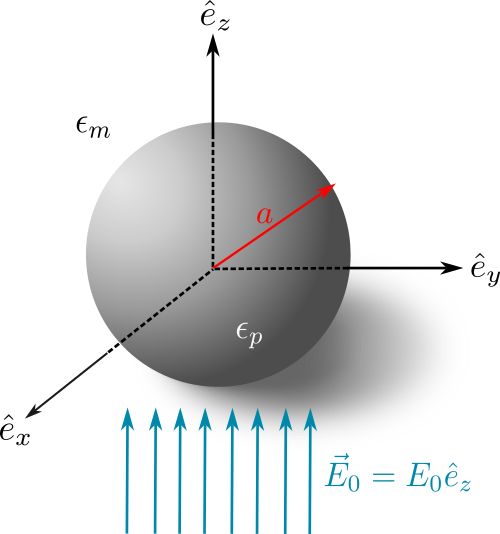
\includegraphics[width=0.3\textwidth]{../../Figuras/shereE0}\label{system}}
		\sidesubfloat[Second image]{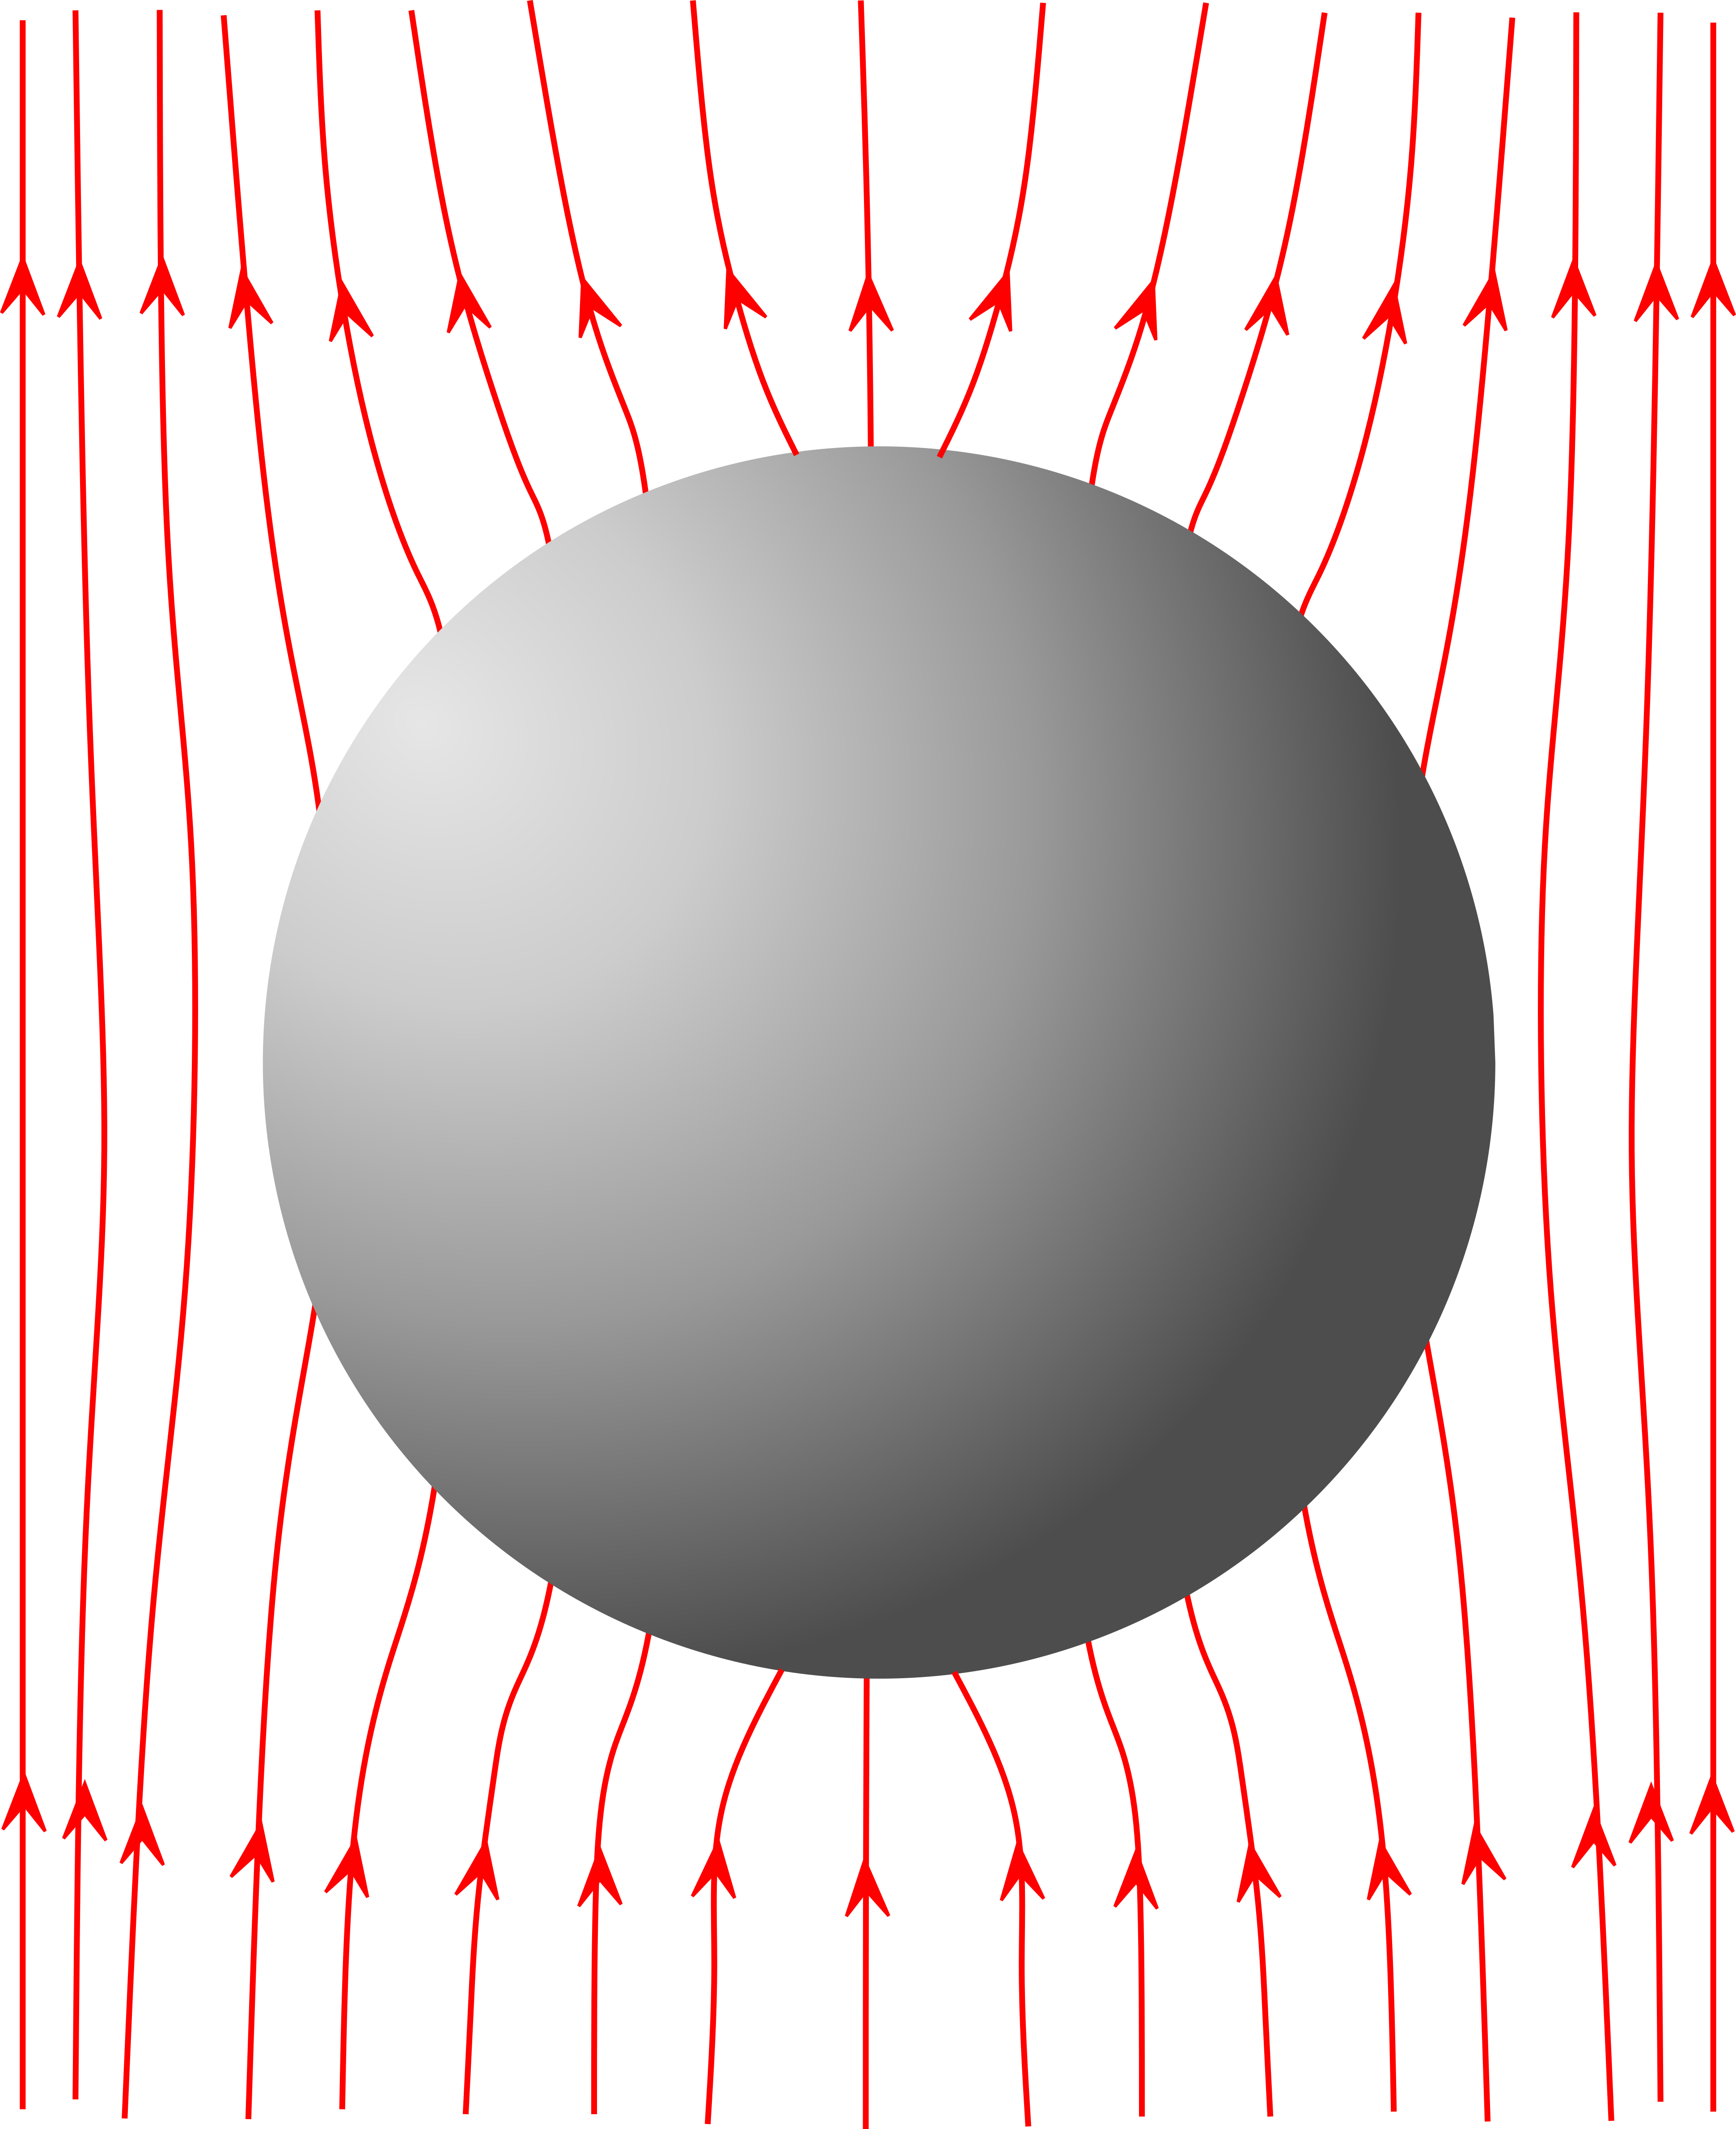
\includegraphics[width=0.25\textwidth]{../../Figuras/electricfield_sphere.png}\label{electricfieldsphere}}
	\caption{Problema de una esfera inmersa en un campo eléctrico homogéneo. \textbf{a)} Esfera de radio $a$ caracterizada por su función dieléctrica $\epsilon_p$ y embebida en un medio caracterizado por su función dieléctrica $\epsilon_m$ en la cual incide un campo eléctrico uniforme $\Vec{E}_0$. \textbf{b)} Campo eléctrico fuera de la esfera generado por la superposición del campo eléctrico aplicado y del campo eléctrico producido por un dipolo eléctrico puntual localizado en el origen con momento dipolar $\vec{p}= \epsilon_m\alpha\Vec{E}_0$.}
	\label{steady_state}
\end{figure}
 

\subsubsection{Dipolo eléctrico (caso dinámico)}

En la sección anterior se abordó una solución que asume que el campo eléctrico externo,  por tanto el dipolo inducido, son estáticos. Para resolver el caso dinámico en el régimen cuasiestático, se considera que, al iluminar cargas confinadas en un volumen finito con una onda plana electromagnética, estas experimentan movimiento. Esto equivale a realizar un análisis en términos de componentes de Fourier de los potenciales y campos generados por un sistema de cargas y corrientes localizadas en el espacio vacío, con una dependencia armónica $e^{-i\omega t}$, tal que varían en el tiempo y oscilan a la frecuencia $\omega$ del campo electromagnético aplicado. De esta forma, la densidad de carga volumétrica  $\rho(\Vec{r},t)$ y la densidad de corriente volumétrica $\Vec{J}(\Vec{r},t)$  en la posición $\Vec{r}$ se expresan como \cite{Jackson}
\begin{align}
    \rho(\Vec{r},t)&=\rho(\Vec{r})e^{-i\omega t},\nonumber\\
    \Vec{J}(\Vec{r},t)&=\Vec{J}(\Vec{r})e^{-i\omega t},
    \label{armonicf}
\end{align}
considerando que el significado físico lo posee la parte real. Mediante lo anterior, es posible determinar los campos electromagnéticos generados por las cargas y corrientes mediante el potencial vectorial como \cite{Jackson}:
\begin{align}
  \Vec{A}(\Vec{r},t)=\frac{\mu_0}{4\pi}\int \left( \text{d}^3r'\frac{\Vec{J}(\Vec{r'})}{|\Vec{r}-\Vec{r'}|}\right)e^{-i\omega t_r},
  \label{Achafa}
\end{align}
en donde se emplea la norma de Lorentz \cite{Griffiths} y la densidad de corriente se evalúa en el tiempo de retardo $t_r=t-|\Vec{r}-\Vec{r'}|/c$. \\

El comportamiento de los campos electromagnéticos se puede estudiar al delimitar diferentes regiones considerando valores extremos de $k=\omega/c$. Empleando la definición anterior y obviando la dependencia temporal, la Ec. (\ref{Achafa}) se reescribe como
\begin{equation}
    \Vec{A}(\Vec{r})=\frac{\mu_0}{4\pi}\int \Vec{J}(\Vec{r'})\frac{e^{ik|\Vec{r}-\Vec{r'}|}}{|\Vec{r}-\Vec{r'}|} \text{d}^3r'.
    \label{pot_vectorial}
\end{equation} 
En la región de campo cercano, donde $r\ll\lambda$ (o $kr\ll 1$), tal que exp($ik|\Vec{r}-\Vec{r'}|)\to 1$, se tiene \cite{Jackson}
\begin{equation*}
	\Vec{A}(\Vec{r},t)=\frac{\mu_0}{4\pi}\int \frac{\Vec{J}(\Vec{r'})}{|\Vec{r}-\Vec{r'}|} \text{d}^3r',
\end{equation*} 
mientras que en la región de campo lejano ($kr\gg 1$) dado que la exponencial oscila rápidamente, es suficiente aproximar
\begin{equation}
	|\Vec{r}-\Vec{r'}|\simeq r-\hat{e}_r\cdot\Vec{r'},    
\end{equation}
 que se obtiene al aplicar la ley de cosenos\footnote{Empleando la ley de cosenos y haciendo una expansión binomial $
 	|\Vec{r}-\Vec{r'}|=\sqrt{r^2+(r')^2-2rr'\cos\theta}=r\sqrt{1+\left(r'/r\right)^2-2\left((r'/r)\cos\theta\right)}\simeq r\left\{1-(\hat{e}_r\cdot\Vec{r'}/r)+1/2\left(r'/r\right)^2\right\}\simeq r-\hat{e}_r\cdot\Vec{r'}.$} en el triángulo mostrado en la Fig.~\ref{vectposi}, donde $\hat{e}_r$ un vector unitario en la dirección de $\Vec{r}$. 	
	Si sólo se consideran los términos que decaen como $r^{-1}$, el inverso de la distancia en la Ec. (\ref{pot_vectorial}) puede ser reemplazado por $r$. Entonces, el potencial vectorial es
	\begin{equation*}
	\lim_{kr\rightarrow\infty}\Vec{A}(\Vec{r})=\frac{\mu_0}{4\pi}\frac{e^{ikr}}{r}\int \Vec{J}(\Vec{r'})e^{-ik\hat{e}_r\cdot\Vec{r'}}\text{d}^3r',    
	\end{equation*}
	que se puede reescribir al realizar la expansión en serie de potencias de la exponencial dentro de la integral de volumen, dando como resultado
	\begin{equation*}
	\lim_{kr\rightarrow\infty}\Vec{A}(\Vec{r})=\frac{\mu_0}{4\pi}\frac{e^{ikr}}{r}\sum_n\frac{(-ik)^n}{n!}\int \Vec{J}(\Vec{r'})(\hat{e}_r\cdot\Vec{r'})^n \text{d}^3r'.    
	\end{equation*}
\begin{figure}[h!]
	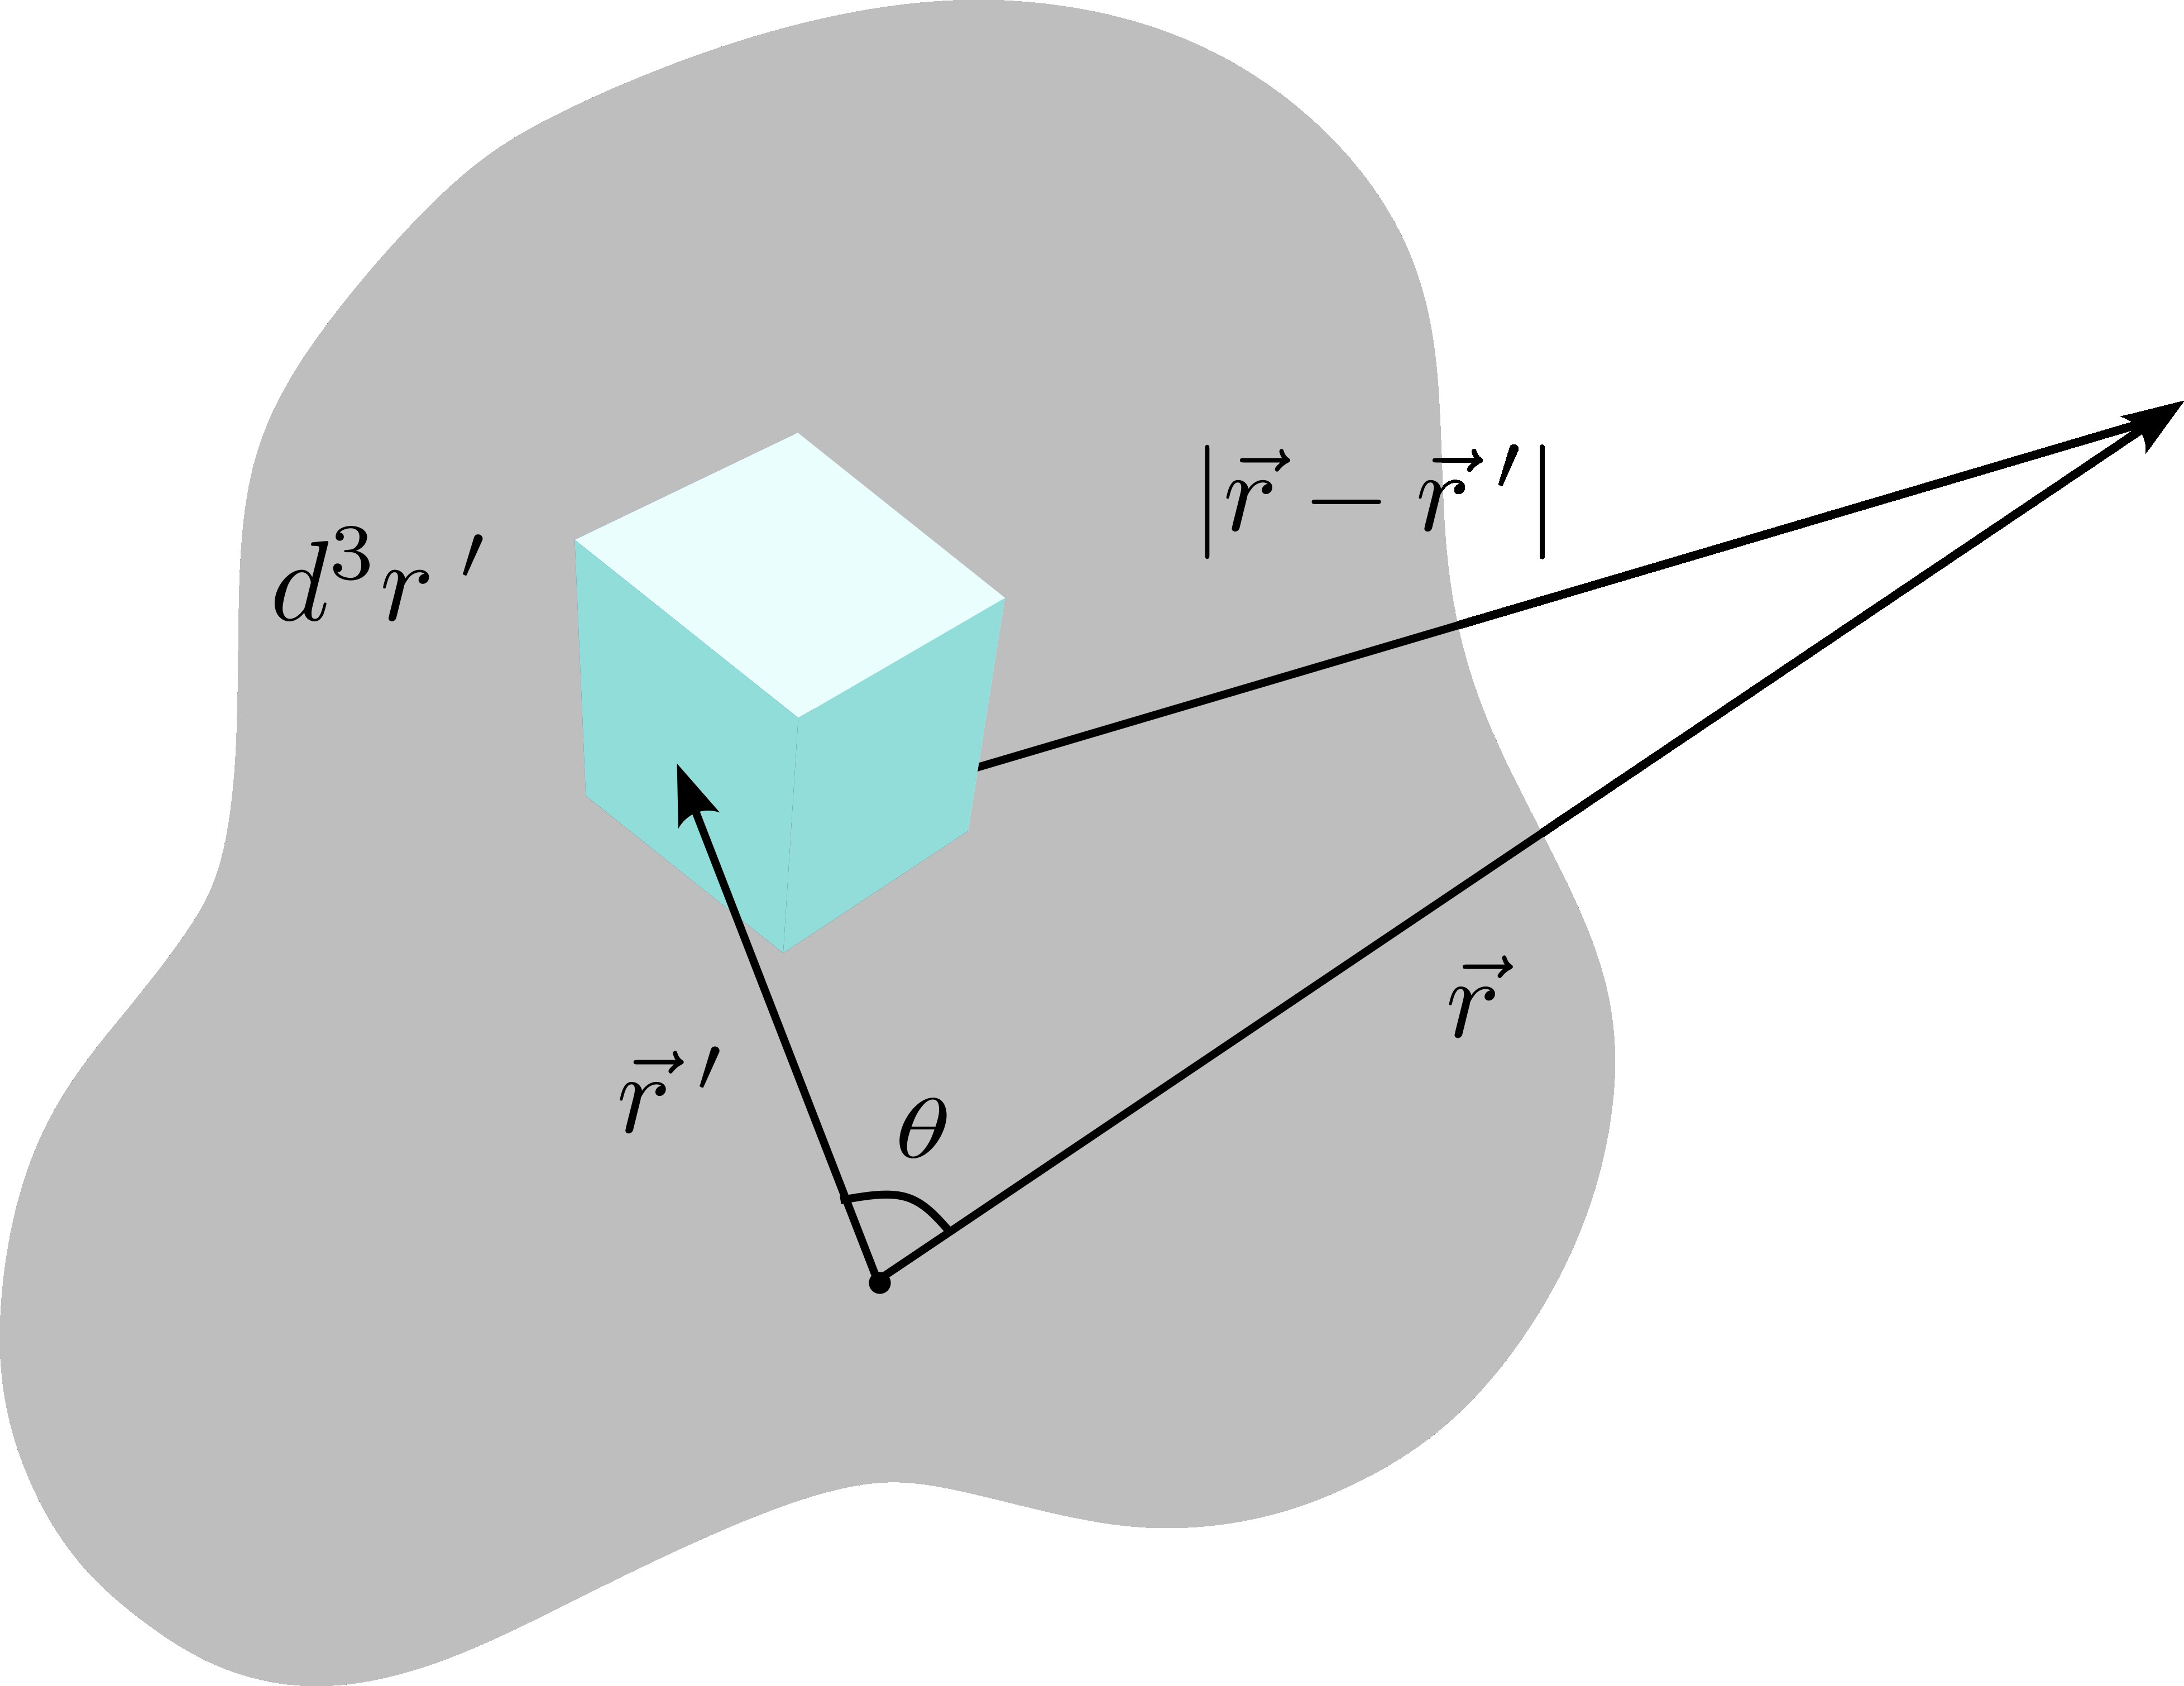
\includegraphics[width=6cm]{../../Figuras/aprox.jpg}
	\caption{Vector de posición $\Vec{r}$ del volumen y $\Vec{r'}$. Se muestra la distancia $|\Vec{r}-\Vec{r'}|$ entre estos últimos. }
	\label{vectposi}
\end{figure}
Al considerar únicamente el primer término de la expansión, se concluye que 
\begin{equation}
    \Vec{A}(\Vec{r})\approx\frac{\mu_0}{4\pi}\frac{e^{ikr}}{r}\int \Vec{J}(\Vec{r'}) \text{d}^3r',    
    \label{aprox_pot_vec}
\end{equation}
que al realizar una integración por partes,  \footnote{Al considerar $\int_V \Vec{r'}(\nabla'\cdot\Vec{J})\text{d}^3r'=\int_{\partial V} \Vec{r'}(\Vec{J}\cdot \text{d}\Vec{S})-\int_V \Vec{J}\text{d}^3r'$ y asumiendo que $\Vec{J}$ se desvanece en los límites del volumen $V$, es decir, en la superficie $\partial V$. } se obtiene que
\begin{equation}
	\int\Vec{J}d^3r'=-\int \Vec{r'}(\nabla'\cdot\Vec{J})\text{d}^3r'=-i\omega\int \Vec{r'}\rho(\Vec{r'})\text{d}^3r',
	\label{Jrho}
\end{equation}
donde se empleó la ecuación de continuidad
\begin{equation*}
    \nabla\cdot\Vec{J}=-\frac{\partial\rho}{\partial t}=i\omega\rho(\Vec{r}). 
\end{equation*}
Al sustituir la Ec. (\ref{Jrho}) en la Ec. (\ref{aprox_pot_vec}) y considerando que el momento dipolar eléctrico $\Vec{p}$ de una distribución de cargas $\rho$ es
\begin{equation*}
	\Vec{p}=\int \Vec{r'}\rho(\Vec{r'})\text{d}^3r',
\end{equation*}
se obtiene 
\begin{equation}
    \Vec{A}(\Vec{r})=-\frac{i\omega\mu_0}{4\pi}\frac{e^{ikr}}{r}\int \Vec{r'}\rho(\Vec{r'})\text{d}^3r'=-\frac{i\omega\mu_0}{4\pi}\frac{e^{ikr}}{r}\Vec{p}. 
    \label{A_dip}  
\end{equation}
Al calcular el campo $\Vec{H}$ como función del potencial vectorial, y empleando la ley de Faraday-Lenz para determinar el campo eléctrico, se sigue que \cite{Jackson}
\begin{align}
	\Vec{E}&=\frac{1}{4\pi\epsilon_0}\left\{k^2(\hat{e}_r\times\Vec{p})\times\hat{e}_r\frac{e^{ikr}}{r}+[3\hat{e}_r(\hat{e}_r\cdot\Vec{p})-\Vec{p}]\left(\frac{1}{r^3}-\frac{ik}{r^2}\right)e^{ikr}\right\},\label{E}\\
    \Vec{H}&=\frac{ck^2}{4\pi}(\hat{e}_r\times\Vec{p})\frac{e^{ikr}}{r}\left(1-\frac{1}{ikr}\right).    \label{H}
\end{align}
A partir de las Ecs. (\ref{E})  y (\ref{H}) se puede observar que el campo $\Vec{H}$ es transversal al vector radial en el campo lejano, mientras el campo eléctrico tiene componentes paralelas y perpendiculares a $\hat{e}_r$.\\ 

 De forma análoga al desarrollo de la Ec. (\ref{A_dip}) y empleando la Ley de Faraday-Lenz, en la zona de radiación cuando $kr\gg 1$, se tiene que al excitar a las fuentes en el sistema con una onda electromagnética de frecuencia angular $\omega$, se induce un dipolo eléctrico $\Vec{p}$ que genera campos electromagnéticos $\Vec{E}_p$ y $\Vec{H}_p$ y  que oscilan a la misma frecuencia $\omega$ 
\begin{align}
    \Vec{E}_p&=\frac{e^{ikr}}{-ikr}\frac{ik^3}{4\pi\epsilon_m}\hat{e}_r\times(\hat{e}_r\times \Vec{p}) e^{i\omega t}, \hspace{1cm}
    \Vec{H}_p=\frac{ck^2}{4\pi}(\hat{e}_r\times\Vec{p})\frac{e^{ikr}}{r}e^{i\omega t}.
\end{align}
En el caso particular en que la onda electromagnética incidente esté polarizada en la dirección $\hat{e}_x$, el momento dipolar inducido es $\Vec{p}=\epsilon_m \alpha E_0 e^{-i\omega t}\hat{e}_x$. Al reescribir al vector en la dirección $\hat{e}_x$ en términos de la base de vectores esféricos como \cite{Griffiths}
\begin{equation}
	\hat{e}_x=\sin\theta\cos\phi\: \hat{e}_r+\cos\theta\cos\phi\: \hat{e}_{\theta}-\sin\phi \:\hat{e}_{\phi},
\end{equation}
se pueden reescribir a los campos generados por el dipolo inducido mediante el vector de amplitud de esparcimiento
\begin{equation}
	\Vec{X}=\frac{ik^3}{4\pi}\alpha \left( \hat{e}_r\times(\hat{e}_r\times \hat{e}_x)\right)=\frac{ik^3}{4\pi}\alpha \left(-\cos\theta\cos\phi \hat{e}_{\theta}+\sin\phi \hat{e}_{\phi} \right),
	\label{Xvec}
\end{equation}
como
 \begin{align}
 	\Vec{E}_{p}&=\frac{e^{ik(r-z)}}{-ikr}\Vec{X}\:E_0 e^{ikz},
 	\hspace{1cm}
 	\Vec{H}_{p}=\frac{k}{\omega\mu}\hat{e}_r\times\Vec{E}_{p}.
 	\label{EH_s}
 \end{align}

